\documentclass[12pt]{article}\usepackage[]{graphicx}\usepackage[svgnames]{xcolor}
%% maxwidth is the original width if it is less than linewidth
%% otherwise use linewidth (to make sure the graphics do not exceed the margin)
\makeatletter
\def\maxwidth{ %
  \ifdim\Gin@nat@width>\linewidth
    \linewidth
  \else
    \Gin@nat@width
  \fi
}
\makeatother

\definecolor{fgcolor}{rgb}{0.345, 0.345, 0.345}
\newcommand{\hlnum}[1]{\textcolor[rgb]{0.686,0.059,0.569}{#1}}%
\newcommand{\hlstr}[1]{\textcolor[rgb]{0.192,0.494,0.8}{#1}}%
\newcommand{\hlcom}[1]{\textcolor[rgb]{0.678,0.584,0.686}{\textit{#1}}}%
\newcommand{\hlopt}[1]{\textcolor[rgb]{0,0,0}{#1}}%
\newcommand{\hlstd}[1]{\textcolor[rgb]{0.345,0.345,0.345}{#1}}%
\newcommand{\hlkwa}[1]{\textcolor[rgb]{0.161,0.373,0.58}{\textbf{#1}}}%
\newcommand{\hlkwb}[1]{\textcolor[rgb]{0.69,0.353,0.396}{#1}}%
\newcommand{\hlkwc}[1]{\textcolor[rgb]{0.333,0.667,0.333}{#1}}%
\newcommand{\hlkwd}[1]{\textcolor[rgb]{0.737,0.353,0.396}{\textbf{#1}}}%
\let\hlipl\hlkwb

\usepackage{framed}
\makeatletter
\newenvironment{kframe}{%
 \def\at@end@of@kframe{}%
 \ifinner\ifhmode%
  \def\at@end@of@kframe{\end{minipage}}%
  \begin{minipage}{\columnwidth}%
 \fi\fi%
 \def\FrameCommand##1{\hskip\@totalleftmargin \hskip-\fboxsep
 \colorbox{shadecolor}{##1}\hskip-\fboxsep
     % There is no \\@totalrightmargin, so:
     \hskip-\linewidth \hskip-\@totalleftmargin \hskip\columnwidth}%
 \MakeFramed {\advance\hsize-\width
   \@totalleftmargin\z@ \linewidth\hsize
   \@setminipage}}%
 {\par\unskip\endMakeFramed%
 \at@end@of@kframe}
\makeatother

\definecolor{shadecolor}{rgb}{.97, .97, .97}
\definecolor{messagecolor}{rgb}{0, 0, 0}
\definecolor{warningcolor}{rgb}{1, 0, 1}
\definecolor{errorcolor}{rgb}{1, 0, 0}
\newenvironment{knitrout}{}{} % an empty environment to be redefined in TeX

\usepackage{alltt}



\usepackage[top=2cm, left=1.2cm, right=1.2cm, bottom=2cm]{geometry} % размер текста на странице


\usepackage{tikz} % картинки в tikz
\usepackage{microtype} % свешивание пунктуации

\usepackage{floatrow} % для выравнивания рисунка и подписи
\usepackage{caption} % для пустых подписей

\usepackage{array} % для столбцов фиксированной ширины

\usepackage{indentfirst} % отступ в первом параграфе

\usepackage{sectsty} % для центрирования названий частей
\allsectionsfont{\centering}

\usepackage{amsmath, amsfonts} % куча стандартных математических плюшек

\usepackage{comment} % для комментариев

\usepackage{multicol} % текст в несколько колонок

\usepackage{lastpage} % чтобы узнать номер последней страницы

\usepackage{enumitem} % дополнительные плюшки для списков
%  например \begin{enumerate}[resume] позволяет продолжить нумерацию в новом списке










\usepackage{fancyhdr} % весёлые колонтитулы
\pagestyle{fancy}
\lhead{Эконометрика, накануне битвы}
\chead{}
\rhead{24.10.2016, демо брутальной части}
\lfoot{}
\cfoot{}
\rfoot{\thepage/\pageref{LastPage}}
\renewcommand{\headrulewidth}{0.4pt}
\renewcommand{\footrulewidth}{0.4pt}



\usepackage{todonotes} % для вставки в документ заметок о том, что осталось сделать
% \todo{Здесь надо коэффициенты исправить}
% \missingfigure{Здесь будет Последний день Помпеи}
% \listoftodos --- печатает все поставленные \todo'шки


% более красивые таблицы
\usepackage{booktabs}
% заповеди из докупентации:
% 1. Не используйте вертикальные линни
% 2. Не используйте двойные линии
% 3. Единицы измерения - в шапку таблицы
% 4. Не сокращайте .1 вместо 0.1
% 5. Повторяющееся значение повторяйте, а не говорите "то же"



\usepackage{fontspec}
\usepackage{polyglossia}

\setmainlanguage{russian}
\setotherlanguages{english}

% download "Linux Libertine" fonts:
% http://www.linuxlibertine.org/index.php?id=91&L=1
\setmainfont{Linux Libertine O} % or Helvetica, Arial, Cambria
% why do we need \newfontfamily:
% http://tex.stackexchange.com/questions/91507/
\newfontfamily{\cyrillicfonttt}{Linux Libertine O}

\AddEnumerateCounter{\asbuk}{\russian@alph}{щ} % для списков с русскими буквами


%% эконометрические сокращения
\DeclareMathOperator{\plim}{plim}
\DeclareMathOperator{\Cov}{Cov}
\DeclareMathOperator{\Corr}{Corr}
\DeclareMathOperator{\Var}{Var}
\DeclareMathOperator{\E}{E}
\def \hb{\hat{\beta}}
\def \hs{\hat{\sigma}}
\def \htheta{\hat{\theta}}
\def \s{\sigma}
\def \hy{\hat{y}}
\def \hY{\hat{Y}}
\def \v1{\vec{1}}
\def \e{\varepsilon}
\def \he{\hat{\e}}
\def \z{z}
\def \hVar{\widehat{\Var}}
\def \hCorr{\widehat{\Corr}}
\def \hCov{\widehat{\Cov}}
\def \cN{\mathcal{N}}


\AddEnumerateCounter{\asbuk}{\russian@alph}{щ} % для списков с русскими буквами
\setlist[enumerate, 2]{label=\asbuk*),ref=\asbuk*}
\IfFileExists{upquote.sty}{\usepackage{upquote}}{}
\begin{document}

\begin{enumerate}

\item Убедитесь, что в рамках классической модели $y=X\beta + u$ и предпосылок $\E(u) = 0$, $\Var(u) = \sigma^2 I$  умеете находить любые $\E()$, $\Var()$ и $\Cov(,)$ для векторов $\beta$, $\hb$, $y$, $\hy$, $u$, $\hat u$.

\item Вектор $u$ размера $4 \times 1$ имеет стандартное нормальное распределение, $u \sim \cN (0; I)$. Известен вектор $d$, $d=(1, -1, 2, -2)$.

\begin{enumerate}
  \item Найдите такую матрицу $H$, что её умноженение на произвольный вектор $y$ означает проецирование вектора $y$ на прямую порождённую вектором $d$
  \item Как распределена случайная величина $u' H u$? Чему равно её математическое ожидание и дисперсия?
\end{enumerate}

\item Вектор $u$ имеет стандартное нормальное распределение, $u \sim \cN (0; I)$. Матрица $A$ такова, что $Au$ также имеет стандартное нормальное распределение, $Au \sim \cN(0;I)$.
\begin{enumerate}
  \item Выпишите уравнение, которому подчиняется матрица $A$
  \item Чему может равняться $\det A$?
  \item Рассмотрим $c_1$ и $c_2$ — первый и второй столбец матрицы $A$. Найдите $c_1'c_1$ и $c_1'c_2$
\end{enumerate}

\item Предположим, что функция $f(x) = x'Ax + Bx + c$ имеет минимум. Найдите его, используя технику дифференциирования по вектору

\item Рассмотрим систему уравнений $X\beta = y$. Здесь $y$ — известный вектор размера $n\times 1$, $\beta$ — неизвестный вектор размера $k\times 1$, и $X$ — известная матрица размера $n\times k$ полного ранга. Мы хотим решить эту систему относительно $\beta$. Если $n=k$, то решать эту систему скучно, и, конечно, $\beta = X^{-1}y$. Гораздо интереснее решать систему, когда решений нет или когда их бесконечно много :)

\begin{enumerate}
\item Если решений нет, то найдите наилучшее приближение к решению, то есть такое $\beta$ при котором длина $(y-X\beta)$ минимальна.
\item Если решений, $\beta$, бесконечно много, то найдите решение с наименьшей длиной.
\end{enumerate}


\end{enumerate}

\begin{figure}[h!]
\floatbox[{\capbeside\thisfloatsetup{capbesideposition={right,bottom},capbesidewidth=4cm}}]{figure}[\FBwidth]
{\caption*{Randall Munroe, xkcd}}
{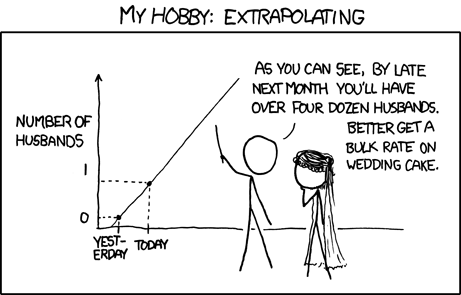
\includegraphics[width=10cm]{extrapolating.png}}
\end{figure}



\end{document}
